\documentclass[a4paper,12pt]{article}
\usepackage[utf8]{inputenc}
\usepackage[T1]{fontenc}
\usepackage[hungarian]{babel}
\usepackage{graphicx}
\usepackage{geometry}
\geometry{a4paper,
		     tmargin = 35mm, 
		     lmargin = 25mm,
		     rmargin = 30mm,
		     bmargin = 30mm}
\usepackage{mathtools}
\usepackage{amsmath}
\usepackage{color}
\usepackage{setspace}
\usepackage{amsmath,amssymb}
\usepackage{float}

\usepackage{indentfirst}
\usepackage{subfig}

\usepackage{siunitx}

\renewcommand\thesection{\Roman{section}}

\begin{document}

\linespread{1.25}

\begin{titlepage}

	\centering
	
\includegraphics[width=0.66\textwidth]{elte.jpg}\par\vspace{1cm}
	{\scshape\LARGE ELTE TTK \par}
	\vspace{3cm}
	{\scshape\Large Kalorimetria \par}
	\vspace{1cm}
	{\large\itshape Olar Alex\par}
	\vspace{3cm}
	{\large 2018 \par}
	
\end{titlepage}

\tableofcontents

\newpage

\section{Elméleti összefoglaló, mérési eszközök}

\vspace{5mm}

\par A mérés során különböző anyagok termodinamikai mennyiségeit vizsgáltuk. Fémüveg kristályosodását, amely egy amorf anyag, ón-ólom ötvözetek olvadását, további para- és ferromágneses fázisátalakulást is. Mindehhez egy DSC\footnote{Differential Scanninc Calorimeter}-t használtunk.

\vspace{5mm}

\par A DSC-ben két kályha fűt egy mintát és egy referenciamintát. A kettőt azonos hőmérsékleten akarjuk tartani, így a laborban található power-compensated (teljesítményfüggő visszacsatolás) DSC ezt csinálja. 

\vspace{5mm}

\par A mért teljesítmény:

\vspace{5mm}

\begin{equation*}
w(T) = (c_{minta} - c_{ref})v + \frac{dh}{dt} + w_{alap}(T)
\end{equation*}

\vspace{5mm}

\par Ahol $c_{minta}, c_{ref}$ rendre a minta és a referencia minta fajhője, $v$ a fűtési sebesség. $\frac{dh}{dt}$ az entalpiaváltozás sebessége, $w_{alap}$, pedig az alapvonal. Az alapvonal egy ismeretlen függvény, amit befolyásol maga a minta, de a kaloriméter is befolyásolja, így nem határozható meg pontosan. Az alapvonalat szabad kézzel szokás behúzni, szemre illesztik. Olvadás esetén a felfutó görbére egyenest illesztve meghatározható az olvadáspont, ami az egyenes és az alapvonal metszéspontja, valamint a függvény és alapvonal közötti területből az olvadáshő is. A kalorimetria legnagyobb problémája az alapvonal, ami miatt nem érthető el nagyon pontos mérés. 

\vspace{5mm}

\par Többkomponensű rendszereknél fennáll egy hőmérséklet-tartomány, amelyen belül a folyadék és szilárd fázis egyszerre van jelen. Ennek vizsgálatára is végeztünk méréséket.

\vspace{5mm}

\par Ezután fémüveget kristályosítottunk át, a felfűtési sebesség, hőfelvétel, és a maximális entalpiaváltozáshoz tartozó hőmérséklet között a következő összefüggés áll fenn.

\vspace{5mm}

\begin{equation*}
lnv = const - 1.052\frac{Q}{RT_{max}}
\end{equation*}

\vspace{5mm}

\par Végül $Ni$ minta para/ferromágneses átalakulását vizsgáltuk a Curie-pont környékén, ahol a fajhő-divergál ($\lambda$-pont).

\newpage

\section{Kiértékelés, eredmények}

\par  Először indium mintát olvasztottunk. Az alapvonalat a program megszerkesztette nekünk, majd egyenest illesztve és a függvény alatti területet kiszámolva, megkaptuk az olvasáspontot ($T = 429.5 ~K$), valamint az olvadáshőt ($L = 27.4 ~J/g$). 

\begin{figure}[H]
\centering
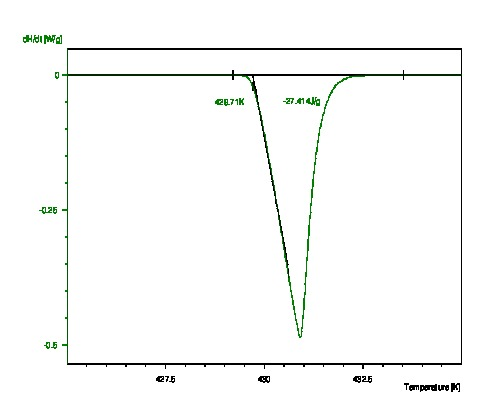
\includegraphics[width=0.7\textwidth]{2outs.jpg}
\end{figure}

\par Továbblépve az ón-ólom ötvözetre. Ennek egy olyan koncentrációjú ötvözetét vizsgáltuk, amely kicsiben tér el attól az ötvözettől, aminek létezik meghatározott olvadáspontja. Így egy olyan görbét láttunk, amin látható, hogy az anyag nagy része egy $T_{0}$ hőmérsékleten megolvad, majd a hőmérséklet növelésével a maradék is fázisátalakuláson megy át. 

\begin{figure}[H]
\centering
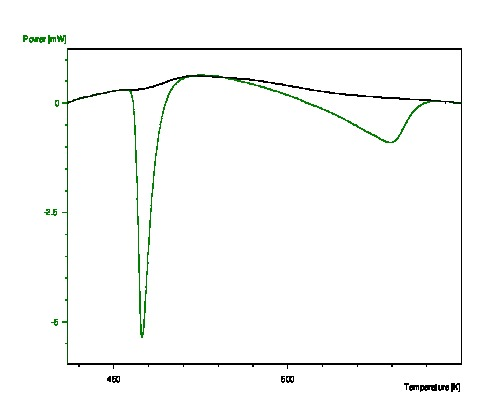
\includegraphics[width=0.6\textwidth]{3outs.jpg}
\end{figure}

\begin{figure}[H]
\centering
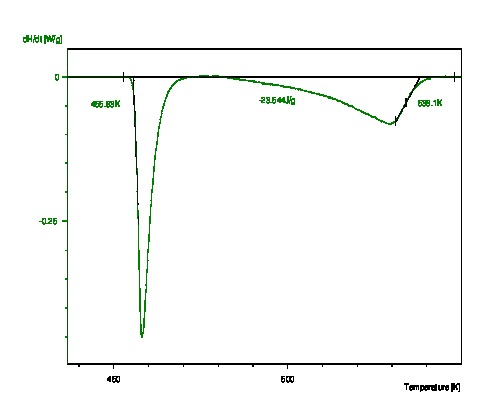
\includegraphics[width=0.55\textwidth]{4outs.jpg}
\end{figure}

\par Az utóbbi ábráról leolvasható $T_{0} = T_{szol} = 455.6 ~K$, ami a szolidusz olvadáspont, valamint $T_{likv} = 538.1 ~K$, ami a likvidusz olvadáspont, ami a második görbe leszállóágára illesztett egyenes és az alapvonal metszéspontjából határozható meg. Mindemellett látható a görbe alatti területből számolt olvadáshő is $L = 25.5 ~J/g$. Az eutektikus pont nagyjából $62 ~m\%/m ~Sn$-nál \footnote{https://www.benbest.com/cryonics/lessons.html} van. Ez az anyag valahol a felett helyezkedik el, nagyjából $70~m\%/m ~Sn$ körül.

\vspace{5mm}

\par Ezután tértünk át a fémüveg átkristályosítására. Ennek során az amorf anyagot addig melegítettük, amíg el nem érte az átkristályosodáshoz szükséges hőmérsékletet. Irreverzibilis folyamat lévén a felfűtést kétszer végeztük el, minden különböző felfűtési sebesség során, majd $ln v ~ \frac{1}{T_{max}}$ összefüggés alapján egyenest véve a következőket kaptuk:

\begin{center}
\begin{tabular}{|c|c|} 
\hline
fűtési sebesség [K/min] & $T_{max}$ [K] \\
\hline
10 & 663.03\\
\hline
20 & 672.2\\
\hline
30 & 680.86\\
\hline
\end{tabular}
\end{center}

\begin{figure}[H]
\centering
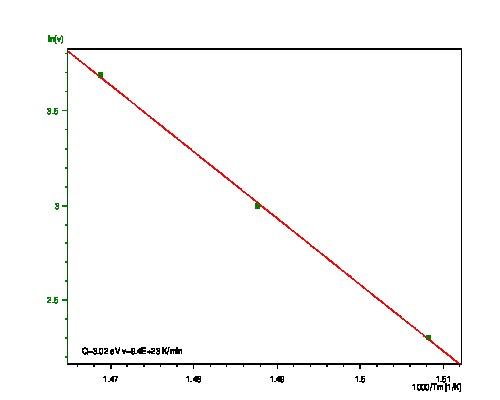
\includegraphics[width=0.5\textwidth]{12outs.jpg}
\end{figure}

\begin{figure}[H]
\centering
\begin{minipage}{0.49\textwidth}
\centering
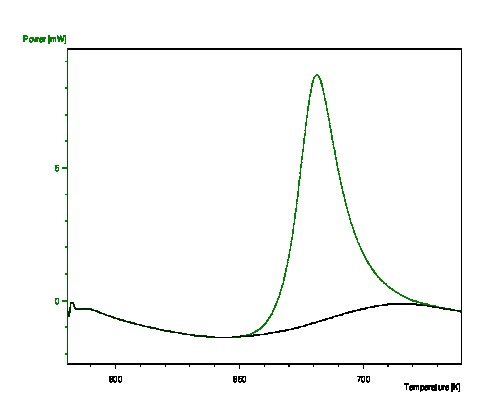
\includegraphics[width=0.8\textwidth]{6outs.jpg}
\end{minipage}
\begin{minipage}{0.49\textwidth}
\centering
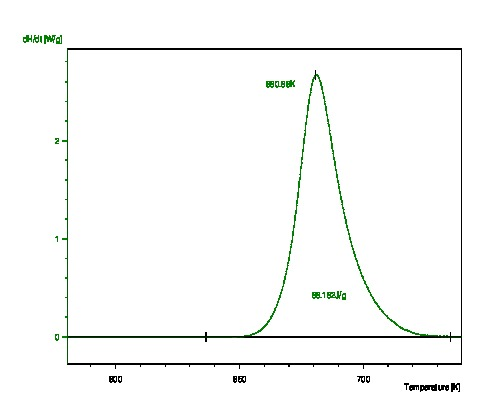
\includegraphics[width=0.8\textwidth]{7outs.jpg}
\end{minipage}
\caption{40 K/min fűtési sebességhez tartozó görbék}
\end{figure}

\begin{figure}[H]
\centering
\begin{minipage}{0.49\textwidth}
\centering
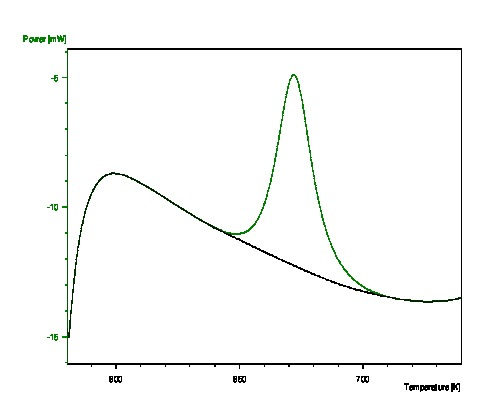
\includegraphics[width=0.8\textwidth]{8outs.jpg}
\end{minipage}
\begin{minipage}{0.49\textwidth}
\centering
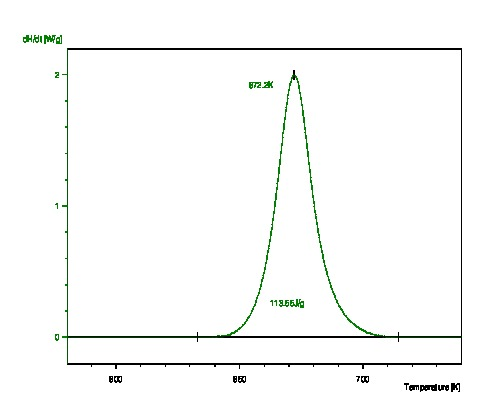
\includegraphics[width=0.8\textwidth]{9outs.jpg}
\end{minipage}
\caption{20 K/min fűtési sebességhez tartozó görbék}
\end{figure}

\begin{figure}[H]
\centering
\begin{minipage}{0.49\textwidth}
\centering
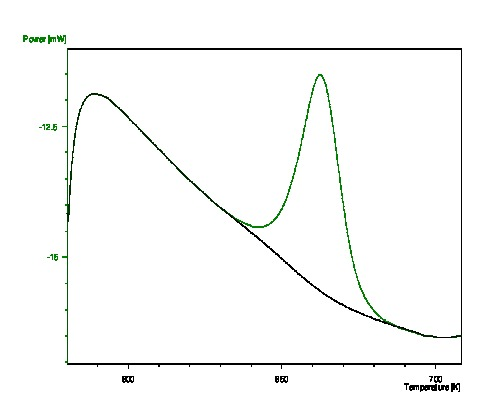
\includegraphics[width=0.8\textwidth]{10outs.jpg}
\end{minipage}
\begin{minipage}{0.49\textwidth}
\centering
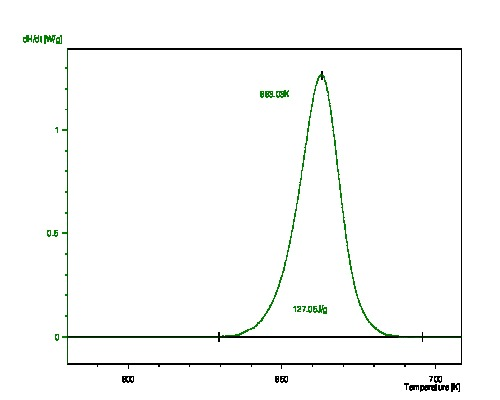
\includegraphics[width=0.8\textwidth]{11outs.jpg}
\end{minipage}
\caption{10 K/min fűtési sebességhez tartozó görbék}
\end{figure}

\par A korábbiakban nem említettem, de természetesen az egyenes alapvonal szoftveresen előállított.

\vspace{5mm}

\par Végül a $Ni$-re tértünk át, aminek mágneses tulajdonságait vizsgáltuk a Curie-pont környékén. Ehhez a modulált kalorimetria módszerét alkalmaztuk, amely során a reverzibilis és irreverzibilis folyamatokat lehet szétválasztani. A felfűtés során egy szinuszos jellel moduláljuk az egyenes felfűtési szakaszt, így a rövid felfűtés során a reverzibilis és irreverzibilis folyamatok is lejátszódnak, míg visszafelé csak a reverzibilisek. Ennek köszönthetően a kapott burkolókból származtathatunk fontos mennyiségeket. A Curie-pont mért értéke $T_{C} = 625.2 ~K$-nek adódott. 

\begin{figure}[H]
\centering
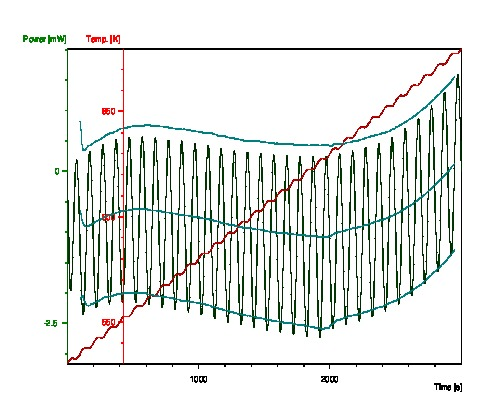
\includegraphics[width=0.6\textwidth]{13outs.jpg}
\end{figure}

\begin{figure}[H]
\centering
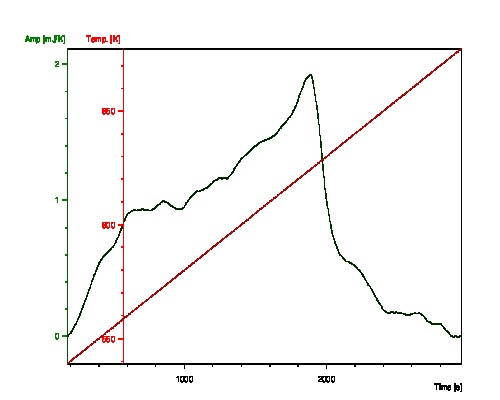
\includegraphics[width=0.6\textwidth]{14outs.jpg}
\caption{ A $\lambda$-pont}
\end{figure}

\section{Összegzés}

\par A mérés sikeresnek tekinthető, mivel a kiértékelt adataink közel egyeznek az irodalmi adatokkal és megismerkedtünk egy viszonylag pontos, ma is használt mérési módszerrel.


\end{document}\grid